\documentclass[notes,11pt, aspectratio=169]{beamer}

\usepackage{pgfpages}
% These slides also contain speaker notes. You can print just the slides,
% just the notes, or both, depending on the setting below. Comment out the want
% you want.
\setbeameroption{hide notes} % Only slide
%\setbeameroption{show only notes} % Only notes
%\setbeameroption{show notes on second screen=right} % Both

\usepackage{helvet}
\usepackage[default]{lato}
\usepackage{array}

\usepackage{subcaption} % for two figures


\usepackage{tikz}
\usepackage{verbatim}
\setbeamertemplate{note page}{\pagecolor{yellow!5}\insertnote}
\usetikzlibrary{positioning}
\usetikzlibrary{snakes}
\usetikzlibrary{calc}
\usetikzlibrary{arrows}
\usetikzlibrary{decorations.markings}
\usetikzlibrary{shapes.misc}
\usetikzlibrary{matrix,shapes,arrows,fit,tikzmark}
\usepackage{amsmath}
\usepackage{mathpazo}
\usepackage{hyperref}
\usepackage{lipsum}
\usepackage{multimedia}
\usepackage{graphicx}
\usepackage{multirow}
\usepackage{graphicx}
\usepackage{dcolumn}
\usepackage{bbm}
\newcolumntype{d}[0]{D{.}{.}{5}}

\usepackage{changepage}
\usepackage{appendixnumberbeamer}
\newcommand{\beginbackup}{
   \newcounter{framenumbervorappendix}
   \setcounter{framenumbervorappendix}{\value{framenumber}}
   \setbeamertemplate{footline}
   {
     \leavevmode%
     \hline
     box{%
       \begin{beamercolorbox}[wd=\paperwidth,ht=2.25ex,dp=1ex,right]{footlinecolor}%
%         \insertframenumber  \hspace*{2ex} 
       \end{beamercolorbox}}%
     \vskip0pt%
   }
 }
\newcommand{\backupend}{
   \addtocounter{framenumbervorappendix}{-\value{framenumber}}
   \addtocounter{framenumber}{\value{framenumbervorappendix}} 
}


\usepackage{graphicx}
\usepackage[space]{grffile}
\usepackage{booktabs}

% These are my colors -- there are many like them, but these ones are mine.
\definecolor{blue}{RGB}{0,114,178}
\definecolor{red}{RGB}{213,94,0}
\definecolor{yellow}{RGB}{240,228,66}
\definecolor{green}{RGB}{0,158,115}

\hypersetup{
  colorlinks=false,
  linkbordercolor = {white},
  linkcolor = {blue}
}


%% I use a beige off white for my background
\definecolor{MyBackground}{RGB}{255,253,218}

%% Uncomment this if you want to change the background color to something else
%\setbeamercolor{background canvas}{bg=MyBackground}

%% Change the bg color to adjust your transition slide background color!
\newenvironment{transitionframe}{
  \setbeamercolor{background canvas}{bg=yellow}
  \begin{frame}}{
    \end{frame}
}

\setbeamercolor{frametitle}{fg=blue}
\setbeamercolor{title}{fg=black}
\setbeamertemplate{footline}[frame number]
\setbeamertemplate{navigation symbols}{} 
\setbeamertemplate{itemize items}{\scriptsize$\blacktriangleright$}

\setbeamercolor{itemize item}{fg=blue}

\setbeamercolor{itemize subitem}{fg=blue}

\setbeamercolor{enumerate item}{fg=blue}
\setbeamercolor{enumerate subitem}{fg=blue}
\setbeamercolor{button}{bg=MyBackground,fg=blue,}



% If you like road maps, rather than having clutter at the top, have a roadmap show up at the end of each section 
% (and after your introduction)
% Uncomment this is if you want the roadmap!
\AtBeginSection[]
 {
    \begin{frame}
        \frametitle{Roadmap of Talk}
        \tableofcontents[currentsection]
    \end{frame}
 }


\setbeamercolor{section in toc}{fg=blue}
\setbeamercolor{subsection in toc}{fg=red}
\setbeamersize{text margin left=1em,text margin right=1em} 

\newenvironment{wideitemize}{\itemize\addtolength{\itemsep}{10pt}}{\enditemize}

\usepackage{environ}
\NewEnviron{videoframe}[1]{
  \begin{frame}
    \vspace{-8pt}
    \begin{columns}[onlytextwidth, T] % align columns
      \begin{column}{.58\textwidth}
        \begin{minipage}[t][\textheight][t]
          {\dimexpr\textwidth}
          \vspace{8pt}
          \hspace{4pt} {\Large \sc \textcolor{blue}{#1}}
          \vspace{8pt}
          
          \BODY
        \end{minipage}
      \end{column}%
      \hfill%
      \begin{column}{.42\textwidth}
        \colorbox{green!20}{\begin{minipage}[t][1.2\textheight][t]
            {\dimexpr\textwidth}
            Face goes here
          \end{minipage}}
      \end{column}%
    \end{columns}
  \end{frame}
}

\title[]{\textcolor{blue}{The Persistent Effects of Peru's Minning Mita \\ Melissa Dell, ECTA 2010} }
\author[PGP]{}
\institute[CUNY]{\small{\begin{tabular}{c}
Jesus Lopez  \\
 The Graduate Center \\ \\

%Author C && Author D   \\
\multicolumn{3}{c}{CUNY} \\
\end{tabular}}}

\date{\today}



\begin{document}
% Title Slide
\begin{frame}
\maketitle
\end{frame}

\section{Motivation}

\begin{frame}{Motivation: Long-term Impacts of Institutions}
    \begin{itemize}
        \item Recent work in economic history leverages a \textbf{big data approach}, focusing on \textbf{sub-national differences} in institutions to understand their long-term impacts.
        \item This approach allows researchers to \textbf{trace back historical events}, analyzing how institutions, even centuries ago, shape modern-day economic outcomes.
        \item By comparing similar regions with varying historical institutional exposure, we can uncover persistent economic effects that would otherwise be difficult to measure.
    \end{itemize}
\end{frame}

\begin{frame}{Motivation: The role of persistence}
        \begin{itemize}
        \item \textbf{Empirical Gap:} Existing evidence provides little clarity on which mechanisms drive the long-term impacts of historical institutions.
        \item \textbf{Potential Mechanisms Explored:}
            \begin{itemize}
                \item Property rights enforcement
                \item Inequality
                \item Ethnic fractionalization
                \item Barriers to entry
                \item Public goods provision
            \end{itemize}
        \item \textbf{Research Focus:} 
            Dell uses variation in the Mining Mita system to identify \textbf{land tenure} (property rights) and \textbf{public goods} as the primary channels through which these effects persist.
    \end{itemize}
\end{frame}

\section{Research question}




% Example slide
\begin{frame}
  \frametitle{What is the research question, why is this important?}
  \begin{itemize}
    \item What are the long-term economic impacts of the Mining Mita system on institutional development and economic outcomes in Peru?
  \end{itemize}
  
\end{frame}


\begin{frame}{Institutional setting: The Mining Mita System (1573–1812)}
  \vspace{3pt}
\begin{columns}[T] % align columns
\begin{column}{.58\textwidth}
\begin{minipage}[t][\textheight][t]
  {\dimexpr\textwidth}
 \vspace{8pt}
      \begin{itemize}
        \item The \textbf{Mining Mita} was a forced labor system implemented by the Spanish colonial government in Peru from \textbf{1573 to 1812}.
        \item Communities near the largest mines, such as Potosí and Huancavelica, were required to send \textbf{1/7th of their adult male population} annually to work in these mines.
        \item This system was intended to \textbf{ensure a steady labor supply for the Spanish silver mining industr}y, essential for colonial economic interests.
    \end{itemize}
    
    \end{minipage}
\end{column}%
\hfill%
\begin{column}{.42\textwidth}
 \colorbox{green!20}{\begin{minipage}[t][1.5\textheight][t]
      {\dimexpr\textwidth}
    \begin{figure}
    \centering
    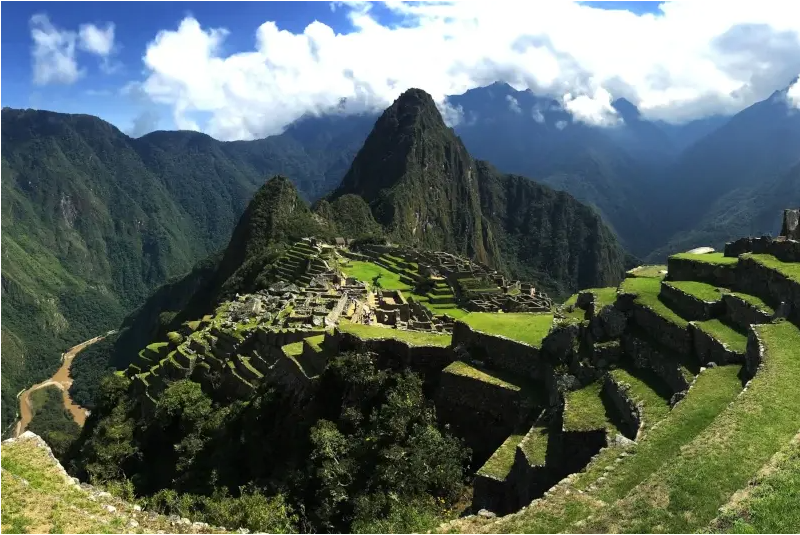
\includegraphics[width=0.8\linewidth]{Picture2.png}
    %\caption{Peru's landscape}
    \label{fig:enter-label}
\end{figure}    \end{minipage}}
\end{column}%
\end{columns}
\end{frame}


\begin{frame}{Institutional setting: Impact of Property Rights and Public Goods Provision}
    \begin{itemize}
        \item \textbf{Property Rights:}
            \begin{itemize}
                \item Non-Mita areas developed clear systems of land ownership and property rights, which persist to this day.
                \item In Mita areas, no clear property rights system emerged after the Mita's end, leaving institutions weaker.
            \end{itemize}
        \item \textbf{Public Goods Provision:}
            \begin{itemize}
                \item Large rural estates in non-Mita areas created employment opportunities and likely advocated for public goods (roads, education).
                \item Dell shows that public goods provision, such as road density, is significantly higher outside Mita boundaries.
            \end{itemize}
    \end{itemize}
\end{frame}


\section{Methodology}

\begin{frame}{What is the methodology? What is novel about this?}
The Spanish government drew a boundary around the mines to limit commuting distances for workers. Only communities \textbf{within this boundary} were required to participate in the Mita labor draft.

    \begin{figure}
        \centering
        \begin{subfigure}{0.45\textwidth} % Adjust the width as needed
            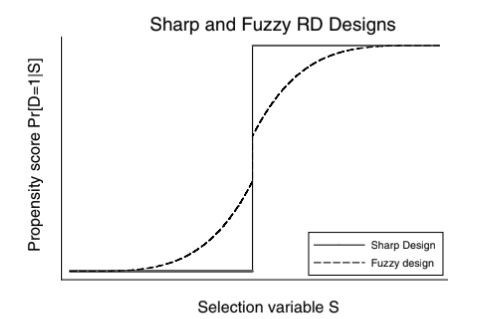
\includegraphics[width=\linewidth]{FigFuzzyDesign.png} % Replace with your image file
            \caption{Classic RD}
        \end{subfigure}
        \hspace{0.05\textwidth} % Adjust horizontal spacing between images
        \begin{subfigure}{0.45\textwidth} % Adjust the width as needed
            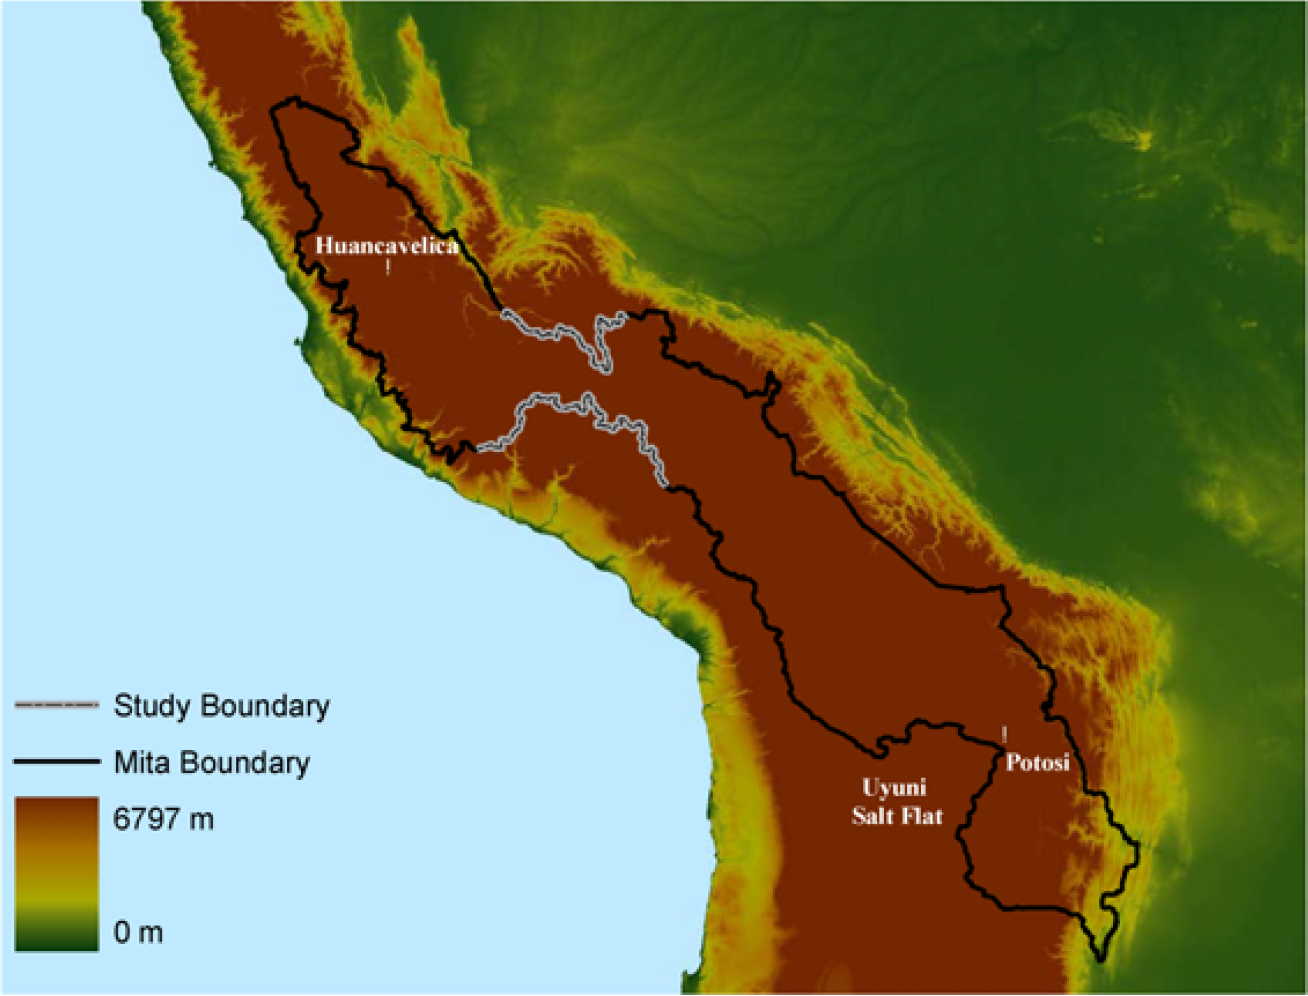
\includegraphics[width=\linewidth]{Picture1.png} % Replace with your image file
            \caption{Spatial RD}
        \end{subfigure}
    \end{figure}
\end{frame}

\begin{frame}{Be careful! Geographic Considerations in Analysis}
    \begin{itemize}
        \item Geographic differences -- such as elevation -- can create distinct economies within and outside the analysis boundary.
        \item Such differences may confound regression discontinuity results, as they introduce other variables affecting economic outcomes beyond the treatment effect.
    \end{itemize}
\end{frame}


\begin{frame}{Addressing Geographic and Economic Challenges}
    \begin{itemize}
        \item \textbf{Focus on Comparable Areas:} Dell selects regions with similar economic conditions before the Mita system to control for pre-existing differences.
        \item \textbf{Data from District Capitals:} She collects data from district capitals inside and outside the Mita region to standardize comparisons and reduce geographic variability.
        \item \textbf{Children’s Heights as an Indicator:} Dell uses children’s heights to assess economic outcomes, providing a tangible measure of health and well-being linked to economic conditions.
        \item  \textbf{Exclusion of Cusco:} Because part of its relative prosperity today likely relates to its pre-mita heritage as the Inca capital (impact is larger when mantained).
    \end{itemize}
\end{frame}




\section{Data}

\begin{frame}{What is the data used?}
    \begin{itemize}
        \item \textbf{Household Consumption Data:}
            \begin{itemize}
                \item From the 2001 Peruvian National Household Survey (ENAHO), collected by the National Institute of Statistics (INEI).
                \item Household consumption is adjusted by subtracting transfers and normalizing prices to Lima metropolitan levels.
            \end{itemize}
        \item \textbf{Children’s Heights Data:}
            \begin{itemize}
                \item Microcensus data from the Ministry of Education, measuring the heights of 6- to 9-year-old school children in the region.
                \item Used as a proxy for long-term living standards and health outcomes.
            \end{itemize}
    \end{itemize}
    \vspace{3mm}
Both datasets georeferenced to the district.
\end{frame}

\begin{frame}{Data}
\begin{itemize}
    \item \textbf{Stunning:} Following international standards, children whose heights are more than 2 standard deviations below their age-specific median are classified as stunted (note: medians and sd calculated by the WHO from an international reference population)
    \item  \textbf{Mean Area Weighted Elevation:} Finally, to obtain controls for exogenous geographic characteristics, of each district by overlaying a map of Peruvian districts on 30 arc second (1 km) resolution elevation data produced by NASA’s Shuttle Radar Topography Mission (SRTM).
\end{itemize}
\end{frame}



\section{Identification Strategy}

\begin{frame}[label=id_strategy]{Identification strategy}

\[
c_{idb} = \alpha + \gamma mita_d + X'_{id} \beta + f(\text{geographic location}_d) + \phi_b + \varepsilon_{ibd}
\]
\pause
where 
\begin{itemize}
    \item $c_{ibd}$ is the outcome variable for observation $i$ in district $d$ along segment $b$ of the mita boundary
    \pause
    \item $mita_d$ is an indicator equal to 1 if district d contributed to the mita and equal to 0 otherwise   
    \pause
    \item  $X_{id}$ is a vector of covariates (mean area weighted elevation and slope for district $d$ and demographic variables giving the number of infants, children, and adults in the household)
    \pause
    \item $f(\text{geographic location}_d)$ is the RD polynomial
    \pause
    \item $\phi_b$ is a set of boundary segment fixed effects that denote which of four equal length segments of the boundary is the closest to the observation’s district capital.
\end{itemize}
\end{frame}

\begin{frame}{Treatment variable at the cutoff}
Need to check for equal means for elevation, terrain ruggedness, soil fertility, rainfall, ethnicity, preexisting settlement patterns, local 1572 tribute (tax) rates, and allocation of 1572 tribute revenues.
\begin{center}
    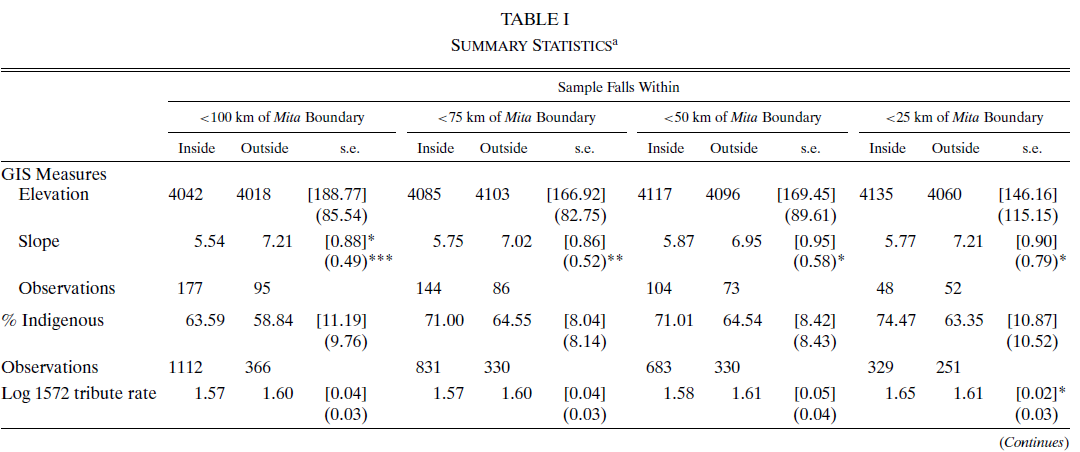
\includegraphics[scale = 0.5]{Picture3a.png}
    \caption{Dell (2010)}
\end{center}
\end{frame}

\begin{frame}{Treatment variable at the cutoff 1}
Need to check for equal means for elevation, terrain ruggedness, soil fertility, rainfall, ethnicity, preexisting settlement patterns, local 1572 tribute (tax) rates, and allocation of 1572 tribute revenues.
\begin{center}
    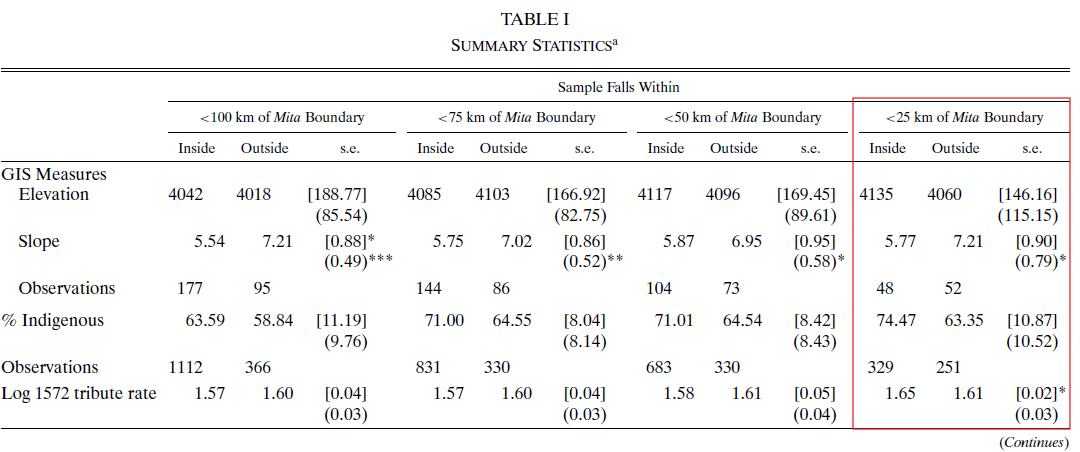
\includegraphics[scale = 0.5]{Picture3b.png}
\end{center}
\end{frame}

\begin{frame}{Treatment variable at the cutoff 2}
    \begin{center}
    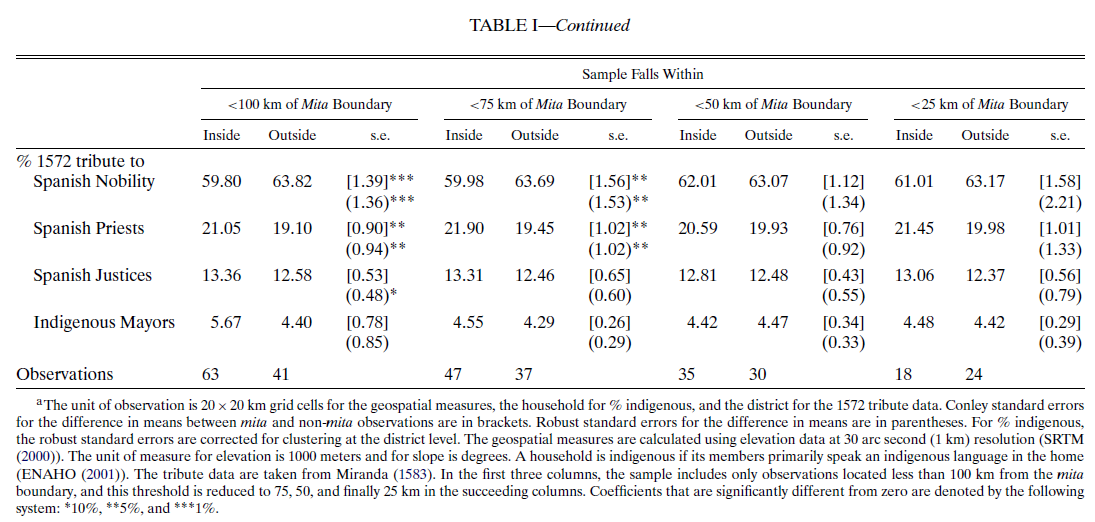
\includegraphics[scale = 0.5]{Picture4a.png}
\end{center}
\end{frame}

\begin{frame}{Treatment variable at the cutoff 2}
    \begin{center}
    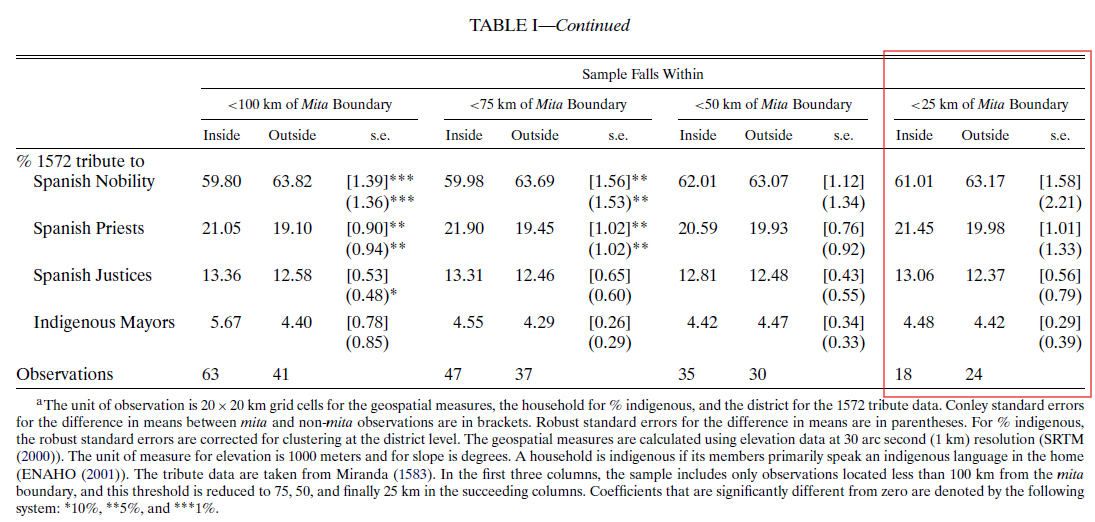
\includegraphics[scale = 0.5]{Picture4b.png}
\end{center}
\end{frame}


\section{Results and discussion}

\begin{frame}{Results}
    \begin{figure}
        \centering
        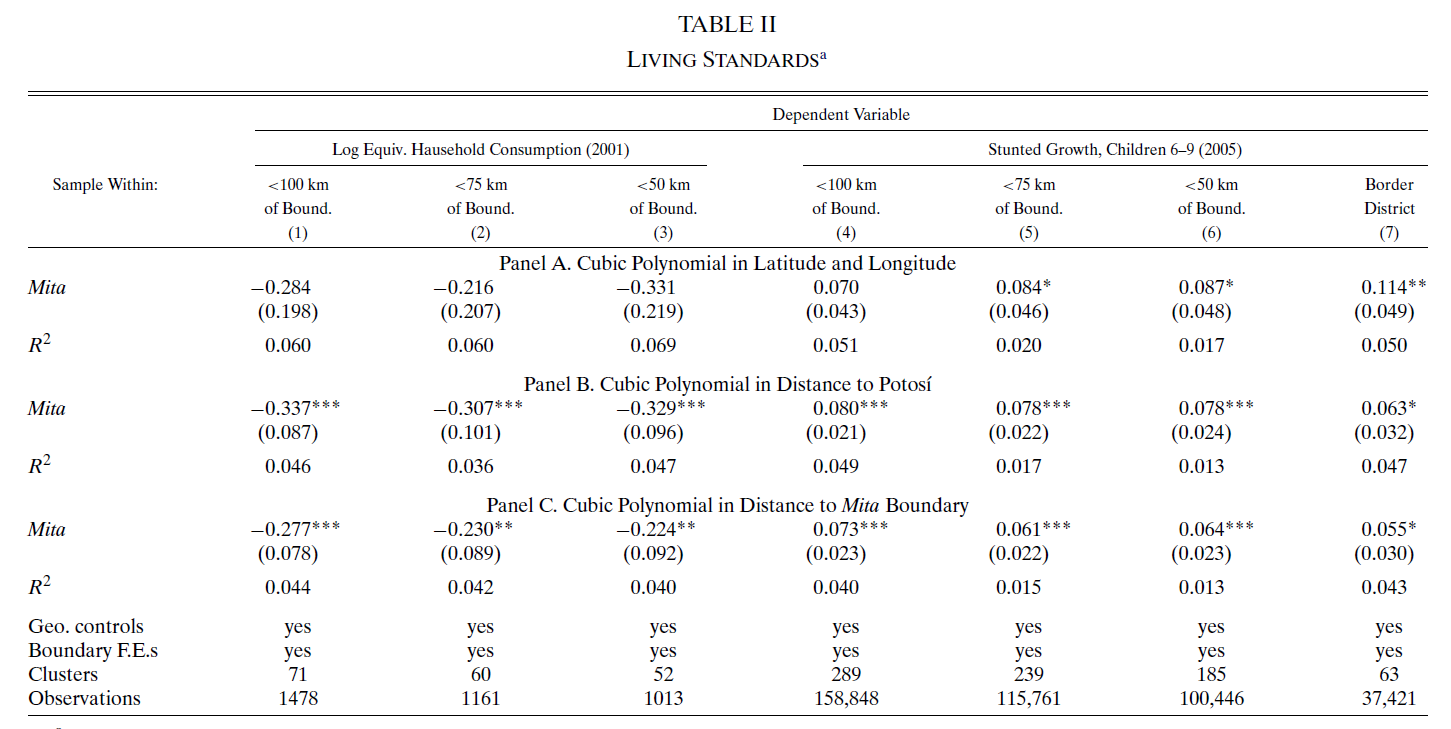
\includegraphics[width=0.8\linewidth]{Table2.png}
        \caption{Dell (2010)}
        \label{fig:enter-label}
    \end{figure}
\end{frame}

\begin{frame}{Results}
    \begin{figure}
        \centering
        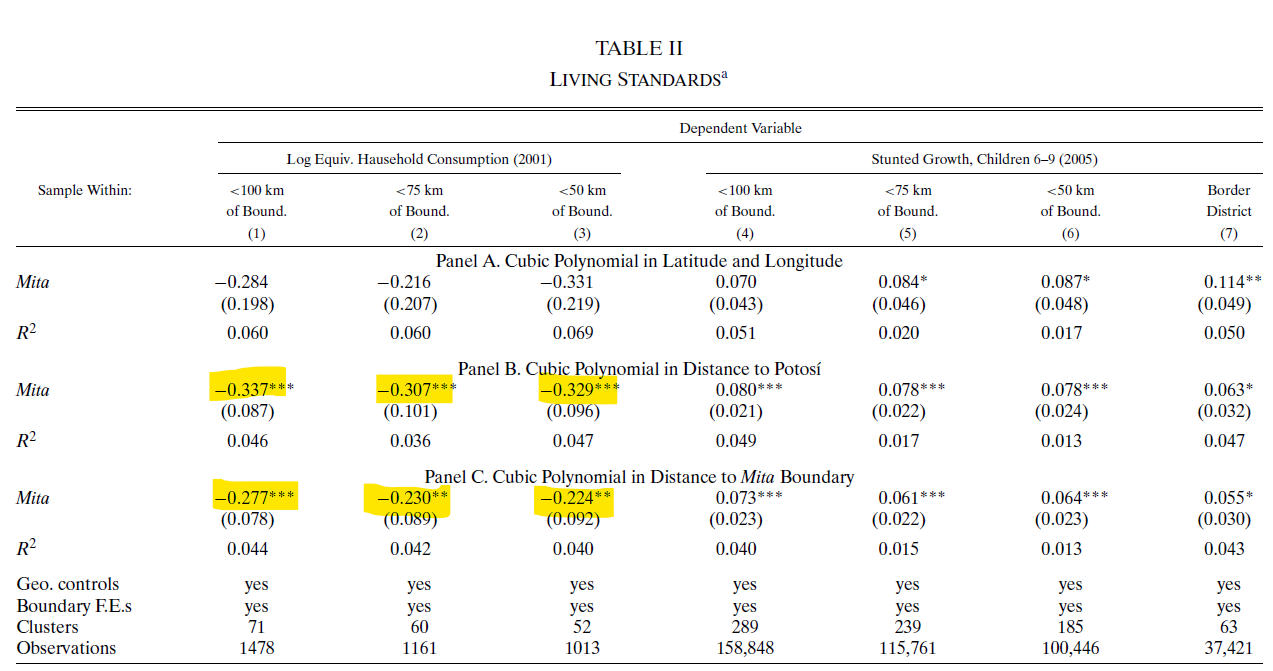
\includegraphics[width=0.8\linewidth]{Table2b.png}
        \caption{Dell (2010)}
        \label{fig:enter-label}
    \end{figure}
\end{frame}

\begin{frame}{Results}
    \begin{figure}
        \centering
        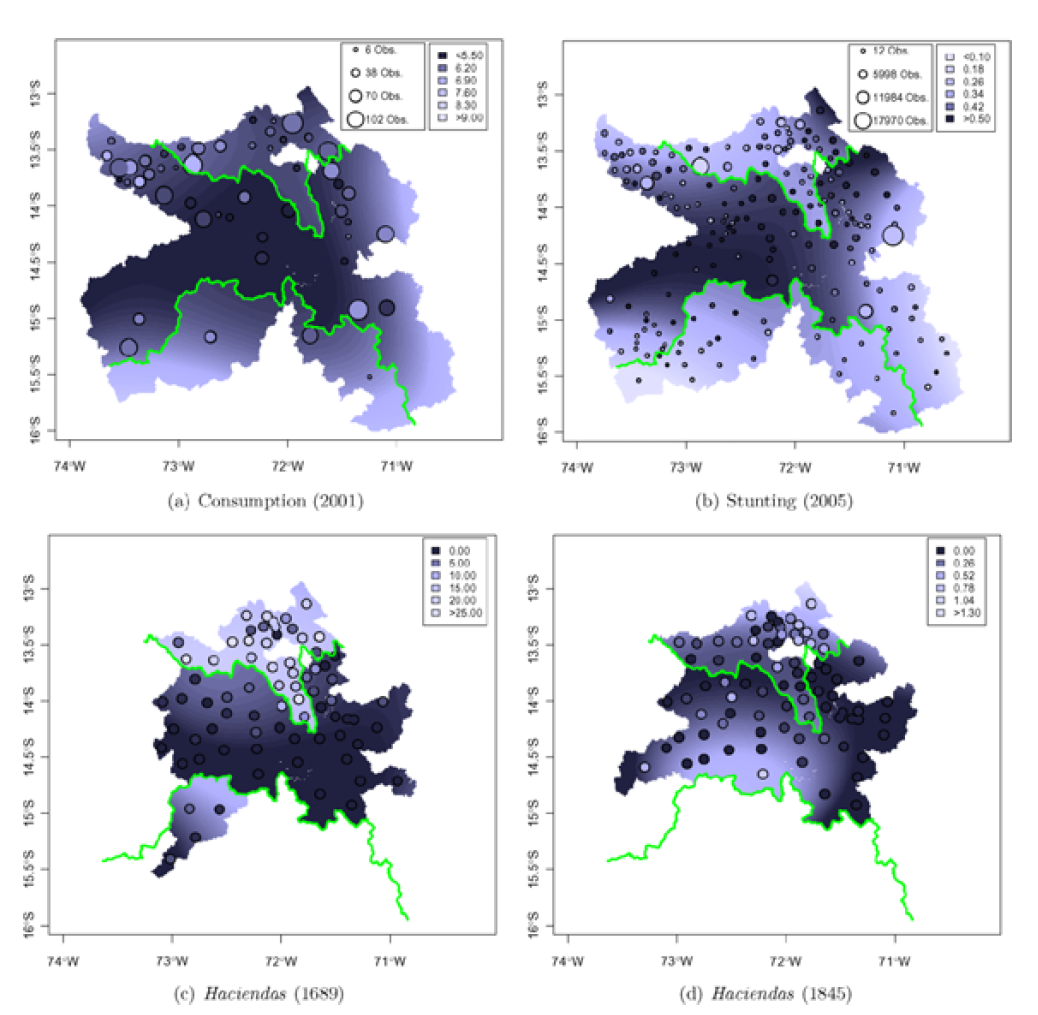
\includegraphics[width=0.45\linewidth]{Picture5.png}
        \caption{Plots of various outcomes against longitude and latitude}
        \label{fig:enter-label}
    \end{figure}
\end{frame}

\begin{frame}{Results}
    \begin{figure}
        \centering
        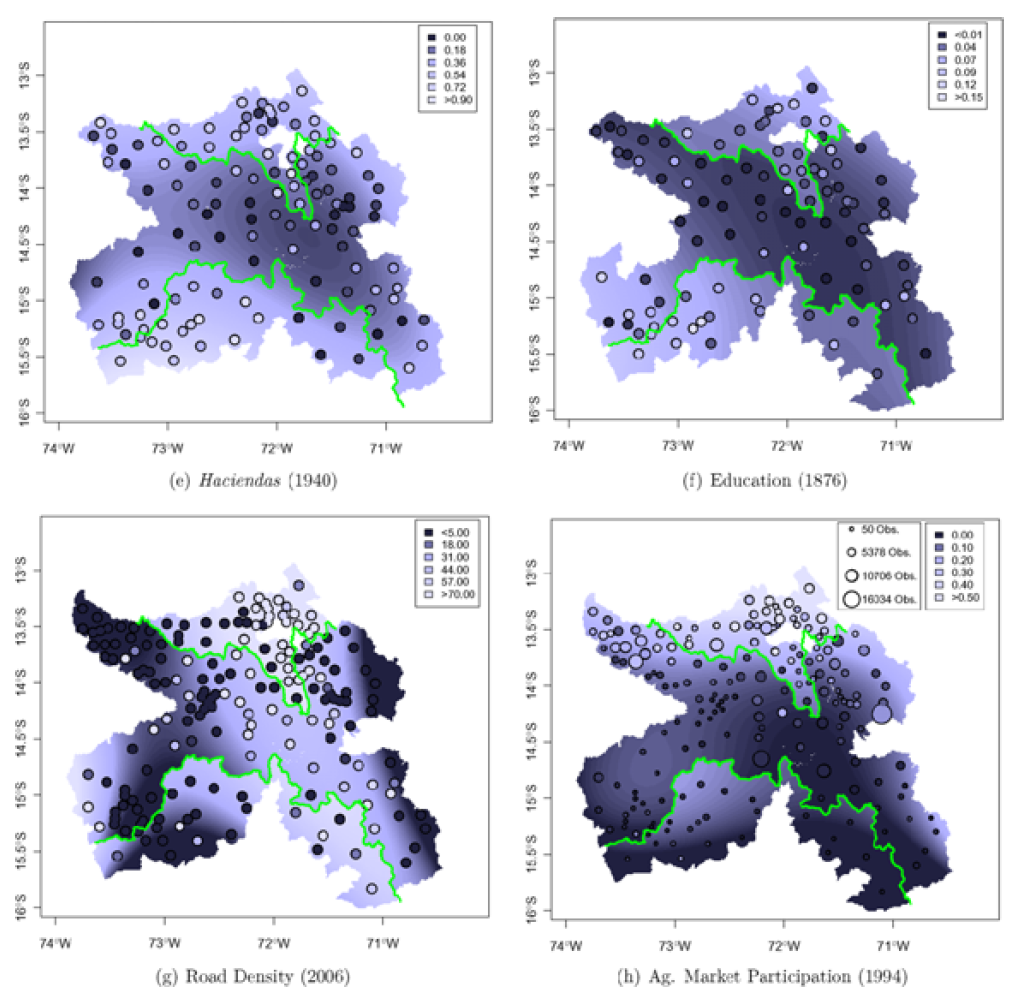
\includegraphics[width=0.45\linewidth]{Picture6.png}
        \caption{Plots of various outcomes against longitude and latitude}
        \label{fig:enter-label}
    \end{figure}
\end{frame}


\begin{frame}{Discussion: Three-Step Process Leading to Institutional Change}
    \begin{enumerate}
        \item \textbf{Impact on Property Rights and Land Ownership:}
            \begin{itemize}
                \item The Mita system weakened property rights in affected areas.
                \item Non-Mita areas developed large estates with formalized ownership, while Mita areas did not.
            \end{itemize}
        \item \textbf{Impact on Public Goods Provision:}
            \begin{itemize}
                \item Large landowners in non-Mita areas advocated for public goods like roads.
                \item Evidence shows roads were built near large farms, reflecting landowner influence.
            \end{itemize}
        \item \textbf{Long-Term Economic Impacts:}
            \begin{itemize}
                \item Disparities in public goods provision altered market structures and productivity.
                \item Mita areas, lacking infrastructure, are still characterized by subsistence farming.
            \end{itemize}
    \end{enumerate}
\end{frame}

\begin{frame}{Persistence}
    \begin{figure}
        \centering
        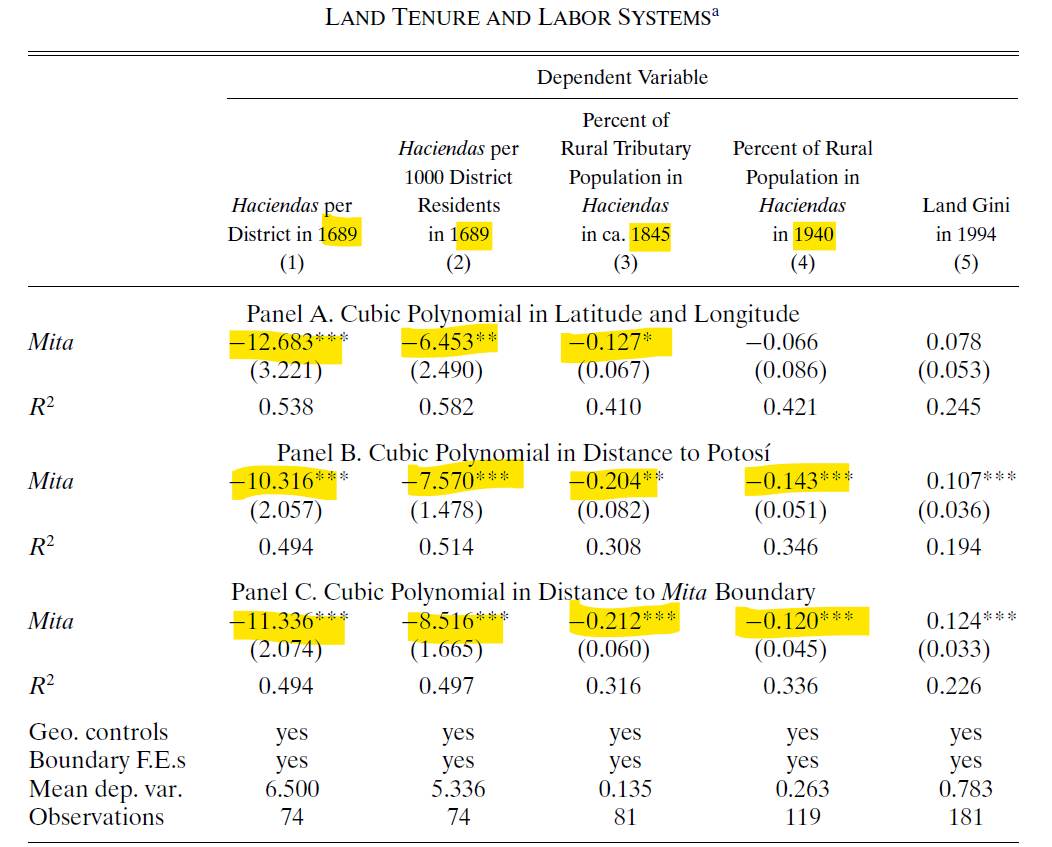
\includegraphics[width=0.6\linewidth]{Table6.png}
        \caption{Land tenure and Labor systems}
        \label{fig:enter-label}
    \end{figure}
\end{frame}



\section{Conclusion and further research}

\begin{frame}{Conclusion 1}
  \begin{itemize}
    \item Outside the mita, owners of ``haciendas'' -- or big farming estates -- used their political clout to have roads built to carry their produce to market.
    \vspace{3mm}
    \item Within the mita, there were fewer haciendas, because the Spanish colonial administration didn’t want competition for labor, and so there were fewer roads.
    \end{itemize}
\end{frame}

\begin{frame}{Conclusions 2}
    \begin{itemize}
        \item \textbf{Role of Large Landowners:}
            \begin{itemize}
                \item Large landowners played a dual role: they did not promote broad economic prosperity, but they shielded individuals from an exploitative state and ensured public goods provision.
            \end{itemize}
        \item \textbf{State Constraints and Economic Interactions:}
            \begin{itemize}
                \item The study highlights that constraints on how the state shapes economic interactions (e.g., coercion of labor, protection of property) are more critical than land inequality for understanding Latin America's long-term growth.
            \end{itemize}
        \item \textbf{Future Research Directions:}
            \begin{itemize}
                \item Future work should focus on the development of general models of institutional evolution and investigate how these constraints are influenced by forces of change.
            \end{itemize}
    \end{itemize}
\end{frame}


\end{document}


